\documentclass[]{article}

\usepackage[utf8]{inputenc}
\usepackage[paperheight=1.5in,paperwidth=2.1in,margin=0in]{geometry}
\usepackage{tikz}
\usetikzlibrary{shapes,arrows,automata,calc}
\usepackage{color}

\usepackage{booktabs}  % nicer table borders 

\begin{document}

%\clearpage
%\thispagestyle{empty}

\tiny{
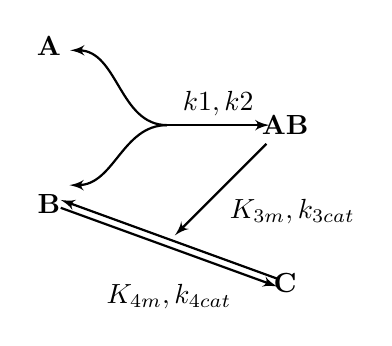
\begin{tikzpicture}[auto, outer sep=0pt, node distance=0cm,>=latex']

\node at (0, 0) (A) {$\bf A$};
\node at (0, -2) (B) {$\bf B$};
\node at (3, -1) (AB) {$\bf AB$};
\node at (1.5, -1) (ABAB) {};
    \draw [->, thick] ($(ABAB)$) to node {$k1, k2$} ($(AB)+(-.2,0)$);
    \path [<-, thick] ($(A.east)+(0,-0.05)$) edge[in=180, out=0] ($(ABAB)$);
    \path [<-, thick] ($(B.north east)$) edge[in=180, out=0] ($(ABAB)$);

    \node at (3, -3) (C) {$\bf C$};
    \draw [<-, thick] ($(B)+(.15,0.05)$) -- ($(C)+(-.1,0.05)$);
    \draw [->, thick] ($(B)+(.15,-0.05)$) to node[below, yshift=-1em] {$K_{4m}, k_{4cat}$} ($(C)+(-.1,-0.05)$);
    \draw [->, thick] (AB) to node {$K_{3m}, k_{3cat}$} ($(C)!0.5!(B)+(0.1,0.1)$);
\end{tikzpicture} 
}

\end{document}

